% Explain the genral stucture of the debugger
The acutal debugger called \emph{Embedded Rust Debugger}(the code for the debugger can be found in the git repository \cite{erd}) consists mainly of two main threads called the \emph{main thead} and the \emph{debug thread}.
The \emph{main thead} is the thread that handels the input from the user from the console or trough \gls{dap} and the \emph{debug thread} handles the reading of \gls{DWARF} information and connection to the debug target.
There is also another thread in the debugger called \emph{input thread} that is only activated if the user is using the console, its jobb is to read the input and send it to the \emph{main thread}.


\subsubsection{The Debug Thread}
% Explain the first state where the debugger is not attach to the debug target
The debug thread has two main state that it changes between, the first state is when it is not attached to any debug target and is called DebugHandler.
The second state is when it is attach to the debug target which means that this state is where debugging can happen, it is called Debugger.


Going back to the fist state, its purpose is to await instructions to attach to the debug target and to receive configuration required for that to happen.
These configurations that the debugger requires is a path to the elf file, a path to the work directory of the code that should be debugged and lastly the type of chip.
When all these are configure the attach command can be used to attach to the micro controller, all the other commands that require that the chip is attach can also be used to attach.


% Explain the second state where the debugger is attach to the debug target.
The debugger uses the library \emph{probe-rs} \cite{probe} to attach to the micro controller and to interact with it.
Thus a lot of useful debugging features like stopping, continuing and setting hardware breakpoints is already given by the \emph{probe-rs} library.
The other features supported by the debugger uses the library \emph{rust-debug} together with the \emph{probe-rs} library.
But the two library are separate so they never interact with each other, the figure \ref{fig:debugger} show how all of these parts interact.
The \emph{rust-debug} library as mention above and seen in the figure \ref{fig:debugger} is a library for retrieving information from the \emph{DWRAF} sections in the \gls{elf} file.
To get some of the information from the library values in the debug targets memory and/or registers are needed.
Thus when calling the \emph{rust-debug} library it can sometimes give a response that says it requires some value from a registry or a memory address, the debugger then uses \emph{probe-rs} to get that value.
Then the read values are sent in to the same \emph{rust-debug} library function as before by storing them in the memory struct that the library uses to read values from the target.
This repeats until the \emph{rust-debug} library returns the requested value or an error if something has gone wrong with reading the \gls{DWARF} format.


\begin{figure}[h]
	\centering
	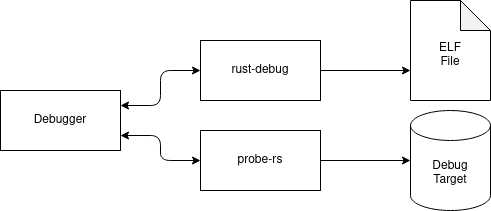
\includegraphics[width=1.0\textwidth]{debugger.png}
	\caption{A diagram showing the relations between the debugger, the \emph{ELF} file, the debug target and the two libraries \emph{rust-debug} and \emph{probe-rs}.}
	\label{fig:debugger}
\end{figure}


\subsubsection{Simultaneous Handling Of Request And Events}
% How the debugger handles request and events simultaneously.
The debug thread polls the channel for incoming request and the state of the debugger.
This enables the debug thread to simultaneously handle requests from the user and events from the debugged target.
There is a boolean that keeps track if the debugged target is running.
It is used to stop the pulling of the targets state when the debugged target is stopped.
This is done because the debugged target cannot start executing on its own,


\subsubsection{Optimization Of Repeated Variable Evaluation}
% How it handles request for stackframes and variables.
To improve on the performance of the debugger the value of the stack frames are stored every time they are calculated.
This allows for fast repetitive look up of information that is stored in the stack frames.
The stored stack frames are removed any time the debugged target starts executing again, thus it will not give old values.


%Also another feature of the debugger is that if the value of a variable is request the debugger will restive all the stack frames instead and then search for the requested variable.
%This simplifies the implementation a lot and will also make the debugger faster when repeated request are made.


\subsubsection{Command Line Interface}
\subimport{}{cli.tex}


\subsubsection{Debug Adapter}
\subimport{}{debug_adapter.tex}

